\documentclass[nohyper,justified]{tufte-handout}\usepackage[]{graphicx}\usepackage[]{color}
%% maxwidth is the original width if it is less than linewidth
%% otherwise use linewidth (to make sure the graphics do not exceed the margin)
\makeatletter
\def\maxwidth{ %
  \ifdim\Gin@nat@width>\linewidth
    \linewidth
  \else
    \Gin@nat@width
  \fi
}
\makeatother

\definecolor{fgcolor}{rgb}{0.345, 0.345, 0.345}
\newcommand{\hlnum}[1]{\textcolor[rgb]{0.686,0.059,0.569}{#1}}%
\newcommand{\hlstr}[1]{\textcolor[rgb]{0.192,0.494,0.8}{#1}}%
\newcommand{\hlcom}[1]{\textcolor[rgb]{0.678,0.584,0.686}{\textit{#1}}}%
\newcommand{\hlopt}[1]{\textcolor[rgb]{0,0,0}{#1}}%
\newcommand{\hlstd}[1]{\textcolor[rgb]{0.345,0.345,0.345}{#1}}%
\newcommand{\hlkwa}[1]{\textcolor[rgb]{0.161,0.373,0.58}{\textbf{#1}}}%
\newcommand{\hlkwb}[1]{\textcolor[rgb]{0.69,0.353,0.396}{#1}}%
\newcommand{\hlkwc}[1]{\textcolor[rgb]{0.333,0.667,0.333}{#1}}%
\newcommand{\hlkwd}[1]{\textcolor[rgb]{0.737,0.353,0.396}{\textbf{#1}}}%

\usepackage{framed}
\makeatletter
\newenvironment{kframe}{%
 \def\at@end@of@kframe{}%
 \ifinner\ifhmode%
  \def\at@end@of@kframe{\end{minipage}}%
  \begin{minipage}{\columnwidth}%
 \fi\fi%
 \def\FrameCommand##1{\hskip\@totalleftmargin \hskip-\fboxsep
 \colorbox{shadecolor}{##1}\hskip-\fboxsep
     % There is no \\@totalrightmargin, so:
     \hskip-\linewidth \hskip-\@totalleftmargin \hskip\columnwidth}%
 \MakeFramed {\advance\hsize-\width
   \@totalleftmargin\z@ \linewidth\hsize
   \@setminipage}}%
 {\par\unskip\endMakeFramed%
 \at@end@of@kframe}
\makeatother

\definecolor{shadecolor}{rgb}{.97, .97, .97}
\definecolor{messagecolor}{rgb}{0, 0, 0}
\definecolor{warningcolor}{rgb}{1, 0, 1}
\definecolor{errorcolor}{rgb}{1, 0, 0}
\newenvironment{knitrout}{}{} % an empty environment to be redefined in TeX

\usepackage{alltt}
\usepackage{mathtools}
%%\usepackage{marginnote}
%%\usepackage[top=1in, bottom=1in, outer=5.5in, inner=1in, heightrounded, marginparwidth=1in, marginparsep=1in]{geometry}
\usepackage{enumerate}
%% mess with the fonts
%%\usepackage{fontspec}
%%\defaultfontfeatures{Ligatures=TeX} % To support LaTeX quoting style
\usepackage[T1]{fontenc}
\usepackage[utf8]{inputenc}
% For package xtable
\usepackage{booktabs}  % Nice toprules and bottomrules
\heavyrulewidth=1.5pt  % Change the default to heavier lines
\usepackage{longtable} 
%%\usepackage{tabularx}  % To control the width of the table

% this should make caption font bold.
%%\usepackage{xstring}
%%\usepackage{etoolbox}

%%\usepackage{url}

%% xetex only \usepackage{breakurl}
\usepackage{float} % for fig.pos='H'
%%\usepackage{wrapfig}
%%\usepackage{tikz}


\usepackage{colortbl,xcolor}
\makeatletter
% Paragraph indentation and separation for normal text
\renewcommand{\@tufte@reset@par}{%
  \setlength{\RaggedRightParindent}{0pc}%
  \setlength{\JustifyingParindent}{0pc}%
  \setlength{\parindent}{0pc}%
  \setlength{\parskip}{3pt}%
}
\@tufte@reset@par

% Paragraph indentation and separation for marginal text
\renewcommand{\@tufte@margin@par}{%
  \setlength{\RaggedRightParindent}{0pc}%
  \setlength{\JustifyingParindent}{0pc}%
  \setlength{\parindent}{0pc}%
  \setlength{\parskip}{2pt}%
}
\makeatother
\makeatletter
\title{Descriptive Statistics -- Associations}
\author{Kate Davis}
\makeatother

\newcommand{\dev}[1] {Dev_{\bar{#1}}}
\IfFileExists{upquote.sty}{\usepackage{upquote}}{}
\begin{document}




\maketitle
\section{Introduction to Associations}
We now consider the statistical associations between data. A data set can contain multiple data points per observation, and understaning how those data are associated within the observation is a key goal of descriptive and inferential statistical analysis. Examples of data sets are observations as patients, with data points as vital signs, or observations as states or counties and data points as crime statistics. 

Some associations that are often examined are statistics including covariance, correlations, and contingencies, and visualizations such as scatterplots and mosaic plots.

\section{US Arrest Statistics by Crime and State}
This data set contains statistics, in arrests per 100,000 residents for assault ($X$) and murder ($Y$) in each of the 50 states in 1973, along with the percent of population living in urban areas ($Z$).


% latex table generated in R 3.1.2 by xtable 1.7-4 package
% Thu Feb 12 19:23:28 2015
\begin{table}[ht]
\centering
\begin{tabular}{rrrr}
  \hline
 & Assault & Murder & UrbanPop \\ 
  \hline
Min. & 45.0 & 0.80 & 32.0 \\ 
  1st Qu. & 109.0 & 4.08 & 54.5 \\ 
  Median & 159.0 & 7.25 & 66.0 \\ 
  Mean & 171.0 & 7.79 & 65.5 \\ 
  3rd Qu. & 249.0 & 11.30 & 77.8 \\ 
  Max. & 337.0 & 17.40 & 91.0 \\ 
  Sum Sq Deviation & 340316.0 & 929.55 & 10266.5 \\ 
  Variance & 6806.3 & 18.59 & 205.3 \\ 
  Standard Deviation & 82.5 & 4.31 & 14.3 \\ 
   \hline
\end{tabular}
\caption{Summary Statistics for US Arrests in 1973 } 
\end{table}

\newpage
\section{Scatterplots}
A \textbf{Scatterplot} of any two of the three variables shows the relationship on the same observation, in this case, State. 
\begin{knitrout}
\definecolor{shadecolor}{rgb}{0.969, 0.969, 0.969}\color{fgcolor}\begin{marginfigure}

{\centering 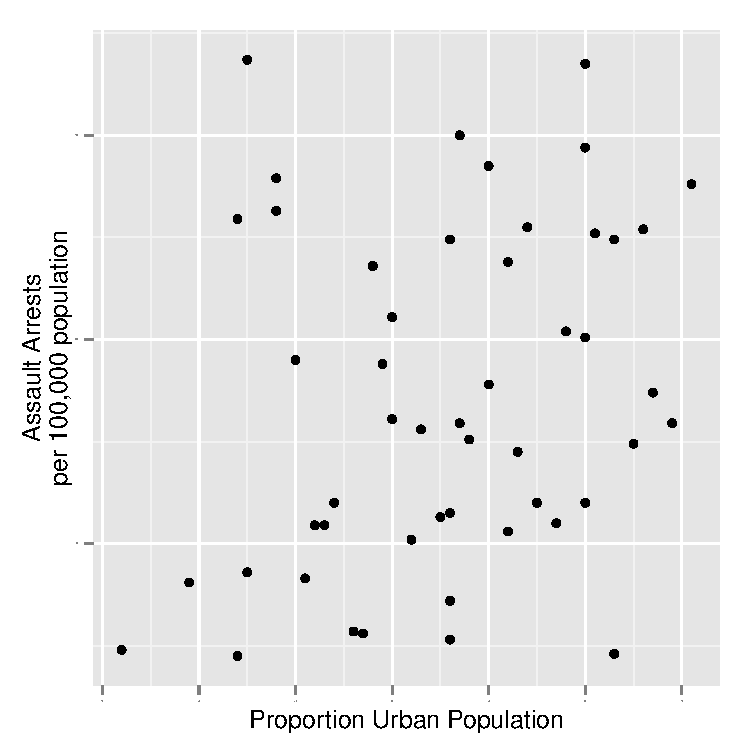
\includegraphics[width=\maxwidth]{figure/graphics-scatterplotsxz-1} 

}

\caption[A scatterplot of Assault Arrests vs]{A scatterplot of Assault Arrests vs. Proportion Urban Population does not show a relationship}\label{fig:scatterplotsxz}
\end{marginfigure}


\end{knitrout}
\begin{knitrout}
\definecolor{shadecolor}{rgb}{0.969, 0.969, 0.969}\color{fgcolor}\begin{marginfigure}

{\centering 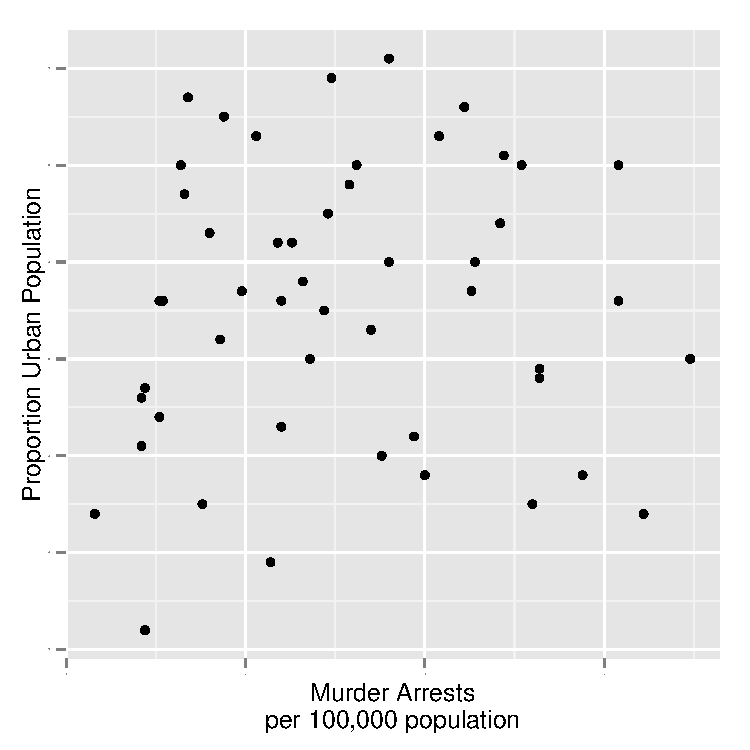
\includegraphics[width=\maxwidth]{figure/graphics-scatterplotsyz-1} 

}

\caption[A scatterplot of Murder Arrests vs]{A scatterplot of Murder Arrests vs. Proportion Urban Population does not show a relationship}\label{fig:scatterplotsyz}
\end{marginfigure}


\end{knitrout}
\begin{knitrout}
\definecolor{shadecolor}{rgb}{0.969, 0.969, 0.969}\color{fgcolor}\begin{figure}

{\centering 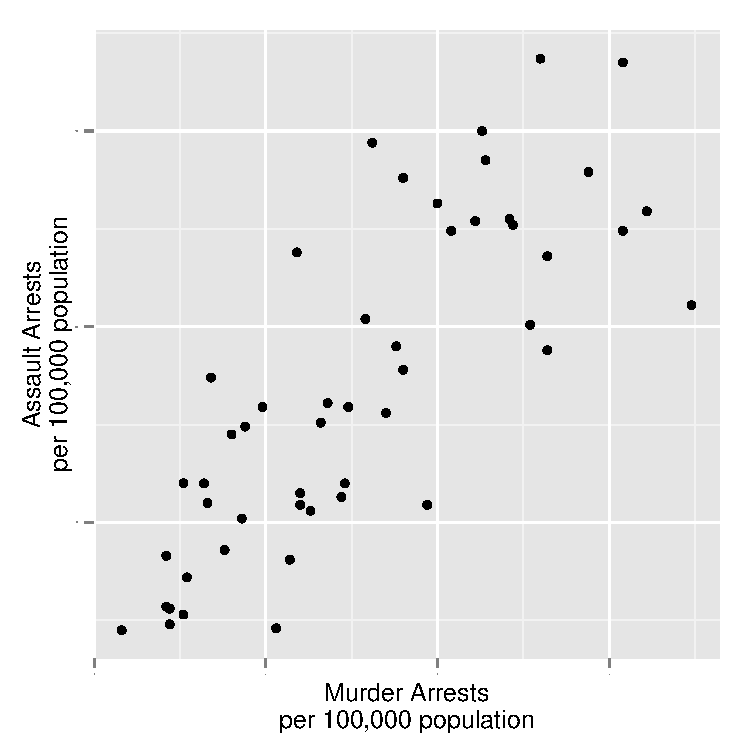
\includegraphics[width=\maxwidth]{figure/graphics-scatterplotsxy-1} 

}

\caption[A scatterplot of Assault vs]{A scatterplot of Assault vs. Murder Arrests shows a possible linear relationship}\label{fig:scatterplotsxy}
\end{figure}


\end{knitrout}
\section{Covariance}
We would like to quantify the linear relationship between each of the variables. The \textbf{Covariance}, a measure of strength of the association between any two variables $X$ and $Y$, denoted $Cov(X,Y)$ is calculated by first multiplying the deviations from their means, $\dev{x}$ and $\dev{y}$, then summing over all observations and dividing by $N$, the number of observations. This is very similar to the population variance calculation, and the variance can be thought of as the covariance of a variable with itself ie. $Var(X)=Cov(X,X)$. 

\begin{equation*}
Cov(X,Y)=Dev_{\bar{x}}*Dev_{\bar{y}}=Dev_{\bar{y}}*Dev_{\bar{x}}=Cov(Y,X)
\end{equation*}
The Covariance of Assault Arrests with Murder Arrests is 285.2416 "Assault Arrests x Murder Arrests". These units make very little sense. We cannot compare covariances among variables in a data set if the units are different.


% latex table generated in R 3.1.2 by xtable 1.7-4 package
% Thu Feb 12 19:23:28 2015
\begin{table}[ht]
\centering
\begin{tabular}{lrrrrrr}
  \toprule
Observation & Assault & Murder & UrbanPop & $\dev{xy}$ & ${\dev{xz}}$ & ${\dev{xz}}$ \\ 
  \midrule
Alabama & 236 & 13.20 &  58 & 351.65 & -487.50 & -40.57 \\ 
   \rowcolor[gray]{0.95}Alaska & 263 & 10.00 &  48 & 203.32 & -1610.00 & -38.67 \\ 
  Arizona & 294 & 8.10 &  80 & 38.13 & 1783.50 & 4.49 \\ 
   \rowcolor[gray]{0.95}Arkansas & 190 & 8.80 &  50 & 19.19 & -294.50 & -15.66 \\ 
  California & 276 & 9.00 &  91 & 127.05 & 2677.50 & 30.86 \\ 
   \rowcolor[gray]{0.95}Colorado & 204 & 7.90 &  78 & 3.63 & 412.50 & 1.38 \\ 
  Connecticut & 110 & 3.30 &  77 & 273.89 & -701.50 & -51.64 \\ 
   \rowcolor[gray]{0.95}Delaware & 238 & 5.90 &  72 & -126.63 & 435.50 & -12.28 \\ 
  Florida & 335 & 15.40 &  80 & 1248.04 & 2378.00 & 110.34 \\ 
   \rowcolor[gray]{0.95}Georgia & 211 & 17.40 &  60 & 384.40 & -220.00 & -52.85 \\ 
  Hawaii &  46 & 5.30 &  83 & 311.25 & -2187.50 & -43.58 \\ 
   \rowcolor[gray]{0.95}Idaho & 120 & 2.60 &  54 & 264.69 & 586.50 & 59.68 \\ 
  Illinois & 249 & 10.40 &  83 & 203.58 & 1365.00 & 45.68 \\ 
   \rowcolor[gray]{0.95}Indiana & 113 & 7.20 &  65 & 34.22 & 29.00 & 0.29 \\ 
  Iowa &  56 & 2.20 &  57 & 642.85 & 977.50 & 47.52 \\ 
   \rowcolor[gray]{0.95}Kansas & 115 & 6.00 &  66 & 100.24 & -28.00 & -0.90 \\ 
  Kentucky & 109 & 9.70 &  52 & -118.42 & 837.00 & -25.78 \\ 
   \rowcolor[gray]{0.95}Louisiana & 249 & 15.40 &  66 & 593.58 & 39.00 & 3.81 \\ 
  Maine &  83 & 2.10 &  51 & 500.72 & 1276.00 & 82.50 \\ 
   \rowcolor[gray]{0.95}Maryland & 300 & 11.30 &  67 & 452.79 & 193.50 & 5.27 \\ 
  Massachusetts & 149 & 4.40 &  85 & 74.58 & -429.00 & -66.10 \\ 
   \rowcolor[gray]{0.95}Michigan & 255 & 12.10 &  74 & 362.04 & 714.00 & 36.63 \\ 
  Minnesota &  72 & 2.70 &  66 & 503.91 & -49.50 & -2.54 \\ 
   \rowcolor[gray]{0.95}Mississippi & 259 & 16.10 &  44 & 731.28 & -1892.00 & -178.67 \\ 
  Missouri & 178 & 9.00 &  70 & 8.47 & 31.50 & 5.45 \\ 
   \rowcolor[gray]{0.95}Montana & 109 & 6.00 &  53 & 110.98 & 775.00 & 22.38 \\ 
  Nebraska & 102 & 4.30 &  62 & 240.81 & 241.50 & 12.21 \\ 
   \rowcolor[gray]{0.95}Nevada & 252 & 12.20 &  81 & 357.21 & 1255.50 & 68.35 \\ 
  New Hampshire &  57 & 2.10 &  56 & 648.66 & 1083.00 & 54.05 \\ 
   \rowcolor[gray]{0.95}New Jersey & 159 & 7.40 &  89 & 4.68 & -282.00 & -9.16 \\ 
   \bottomrule
\end{tabular}
\caption{Covariances, Part 1} 
\end{table}


\newpage
% latex table generated in R 3.1.2 by xtable 1.7-4 package
% Thu Feb 12 19:23:28 2015
\begin{table}[ht]
\centering
\begin{tabular}{lrrrrrr}
  \toprule
Observation & Assault & Murder & UrbanPop & $\dev{xy}$ & ${\dev{xz}}$ & ${\dev{xz}}$.1 \\ 
  \midrule
New Mexico & 285 & 11.40 &  70 & 411.54 & 513.00 & 16.25 \\ 
   \rowcolor[gray]{0.95}New York & 254 & 11.10 &  86 & 274.73 & 1701.50 & 67.85 \\ 
  North Carolina & 337 & 13.00 &  45 & 864.86 & -3403.00 & -106.80 \\ 
   \rowcolor[gray]{0.95}North Dakota &  45 & 0.80 &  44 & 880.74 & 2709.00 & 150.28 \\ 
  Ohio & 120 & 7.30 &  75 & 24.99 & -484.50 & -4.66 \\ 
   \rowcolor[gray]{0.95}Oklahoma & 151 & 6.60 &  68 & 23.80 & -50.00 & -2.98 \\ 
  Oregon & 159 & 4.90 &  67 & 34.68 & -18.00 & -4.33 \\ 
   \rowcolor[gray]{0.95}Pennsylvania & 106 & 6.30 &  72 & 96.85 & -422.50 & -9.69 \\ 
  Rhode Island & 174 & 3.40 &  87 & -13.17 & 64.50 & -94.39 \\ 
   \rowcolor[gray]{0.95}South Carolina & 279 & 14.40 &  48 & 713.88 & -1890.00 & -115.68 \\ 
  South Dakota &  86 & 3.80 &  45 & 339.15 & 1742.50 & 81.80 \\ 
   \rowcolor[gray]{0.95}Tennessee & 188 & 13.20 &  59 & 91.97 & -110.50 & -35.16 \\ 
  Texas & 201 & 12.70 &  80 & 147.30 & 435.00 & 71.19 \\ 
   \rowcolor[gray]{0.95}Utah & 120 & 3.20 &  80 & 234.09 & -739.50 & -66.55 \\ 
  Vermont &  48 & 2.20 &  32 & 687.57 & 4120.50 & 187.26 \\ 
   \rowcolor[gray]{0.95}Virginia & 156 & 8.50 &  63 & -10.65 & 37.50 & -1.77 \\ 
  Washington & 145 & 4.00 &  73 & 98.54 & -195.00 & -28.43 \\ 
   \rowcolor[gray]{0.95}West Virginia &  81 & 5.70 &  39 & 188.10 & 2385.00 & 55.38 \\ 
  Wisconsin &  53 & 2.60 &  66 & 612.42 & -59.00 & -2.59 \\ 
   \rowcolor[gray]{0.95}Wyoming & 161 & 6.80 &  60 & 9.90 & 55.00 & 5.45 \\ 
   \bottomrule
Total & 8538.0 & 389.4 & 3277.0 & 14262.1 & 15301.0 & 214.9 \\ 
\rowcolor[gray]{0.95}Total/N & 171.0 &  7.8 & 65.5 & 285.2 & 306.0 &  4.3 \\ 
 & $\bar{x}$ & $\bar{y}$ & $\bar{z}$ & $Cov(X,Y)$ & $Cov(X,Z)$ & $Cov(Y,Z)$   \\
\end{tabular}
\caption{Covariances, Part 2} 
\end{table}

\newpage
\section{Linear Correlation}

A standardized Covariance is the \textbf{Linear Correlation}, calculated by dividing each Covariance by the Standard Deviations of each of the variables:

\begin{equation*}
Corr(X,Y)=Cov(Y,X)/(StdDev(X)StdDev(Y))=
\end{equation*}

The Correlation of Assault Arrests with Murder Arrests is 0.80187 with no units, so the correlations of multiple pairs of variables can be compared.

Correlations are always between $-1$ and $1$, and are a quantification of the linear relationship between two variables. A correlation of zero means that there is linear relationship between two variables, although there may be a non-linear relationship. A correlation of $1$ or $-1$ is indicates a perfect positive or negative linear relationship. $Corr(X,X)=1$ always.

\textbf{Correlation does not imply Causation!} Even if two variables have a high or perfect correlation, there is not necessarily causation. Causation means X depends on Y or Y depends on X. 

\begin{knitrout}
\definecolor{shadecolor}{rgb}{0.969, 0.969, 0.969}\color{fgcolor}
\begin{figure}
{\centering 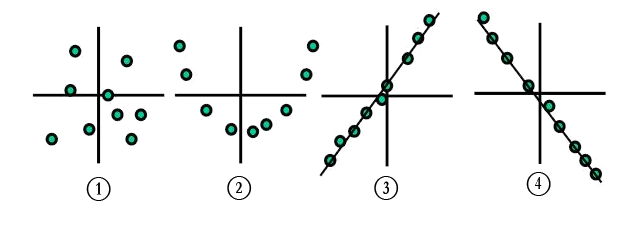
\includegraphics[width=\maxwidth]{Correlation_types-Language-neutral.png} 
}
\caption[Correlation Types]{Examples of Correlation }\label{fig:correlationtypes}
\end{figure}
\textcircled{1} $Corr(X,Y)=0$ No Correlation \\
\textcircled{2} $Corr(X,Y)=0$ No Linear Correlation \\
\textcircled{3} $Corr(X,Y) approaching +1$ Positive Linear Correlation \\
\textcircled{4} $Corr(X,Y) approaching -1$ Negative Linear Correlation\\
\end{knitrout}

The Squared value of the correlation, 64.3\%  is a measure of the "shared variance" of two variable, and the complement 35.7\% is the proportion of variance not explained by the association.
\newpage
\section{Covariance and Correlation Extras}
The covariance relationship between multiple variables can be expressed in a variance-covariance matrix:

\bordermatrix{   ~ & X & Y & Z\cr
                  X & Var(X) & Cov(X,Y) & Cov(X,Z) \cr
                  Y & Cov(Y,X)  & Var(Y) & Cov(Y,Z)  \cr
                  Z & Cov(Z,X)  & Cov(Z,Y)  & Var(Z)}
=
\bordermatrix{   ~ & X & Y & Z\cr
                  X & 6806.32 & 285.2416 & 306.02 \cr
                  Y & 285.2416  & 18.59106 & 4.2984  \cr
                  Z & 306.02  & 4.2984  & 205.33
}

The Variance-Covariance Matrix (also referred to as the VCV or simply the Covariance matrix) is a key part of multivariate statistics and methods, including:
\begin{itemize}
  \item Principal Components Analysis (PCA)
  \item Factor Analysis
  \item Hierarchical Clustering
\end{itemize}

Similarly, the correlation matrix expresses all the correlations among variables.

\bordermatrix{   ~ & X & Y & Z\cr
                  X & Corr(X,X) & Corr(X,Y) & Corr(X,Z) \cr
                  Y & Corr(Y,X)  & Corr(Y,Y) & Corr(Y,Z)  \cr
                  Z & Corr(Z,X)  & Corr(Z,Y)  & Corr(Y,Y)}
=
\bordermatrix{   ~ & X & Y & Z\cr
                  X & 1 & 0.80187 & 0.25886 \cr
                  Y & 0.80187  & 1 & 0.06957  \cr
                  Z & 0.25886  & 0.06957  & 1}

The Correlation Matrix is a key part of multivariate statistics and methods, including:
\begin{itemize}
  \item Canonical Correlation Analysis
  \item Portfolio Analysis and Optimization
\end{itemize}
\begin{knitrout}
\definecolor{shadecolor}{rgb}{0.969, 0.969, 0.969}\color{fgcolor}\begin{figure}

{\centering 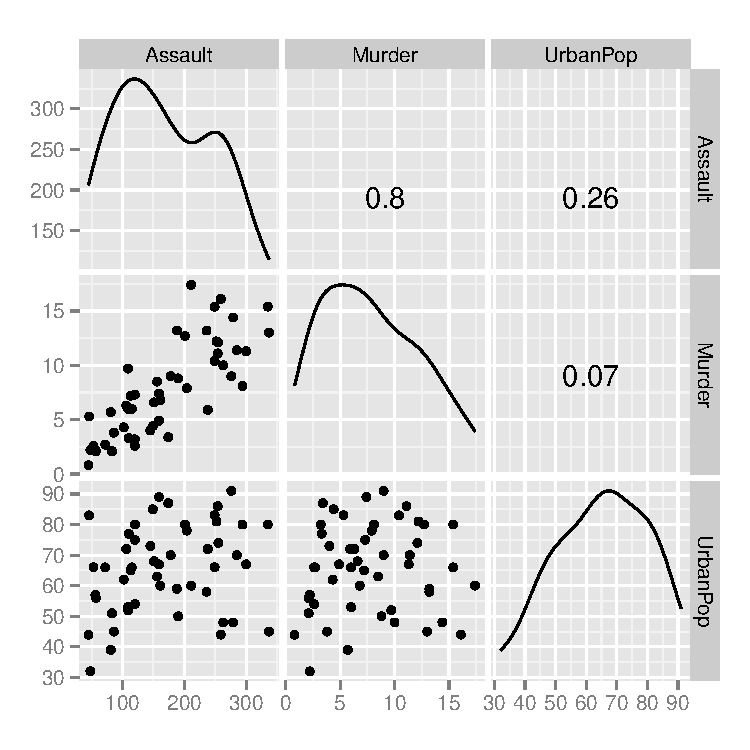
\includegraphics[width=\maxwidth]{figure/graphics-scatmat-1} 

}

\caption[Scatterplot Matrix]{Scatterplot Matrix: Multiple scatterplots and correlations can be combined in one visualization }\label{fig:scatmat}
\end{figure}


\end{knitrout}

When two variables have very different distributions, two non-parametric methods can assess the association on the ranks of the variables: $\rho$, the Spearman Rank Correlation, and $\tau$, the Kendall Rank Correlation.
\newpage
\section{Simple Linear Regression}

When a linear correlation exists between two variables, we can explore causation using a \textbf{Simple Linear Regression}, also called Ordinary Least Squares (OLS), regressing a dependent variable, denoted $Y$, on an independent variable, denoted $X$ as a line with the form:
\begin{equation*}
Y=\alpha + \hat{\beta}X
\end{equation*}
\begin{knitrout}
\definecolor{shadecolor}{rgb}{0.969, 0.969, 0.969}\color{fgcolor}\begin{marginfigure}

{\centering 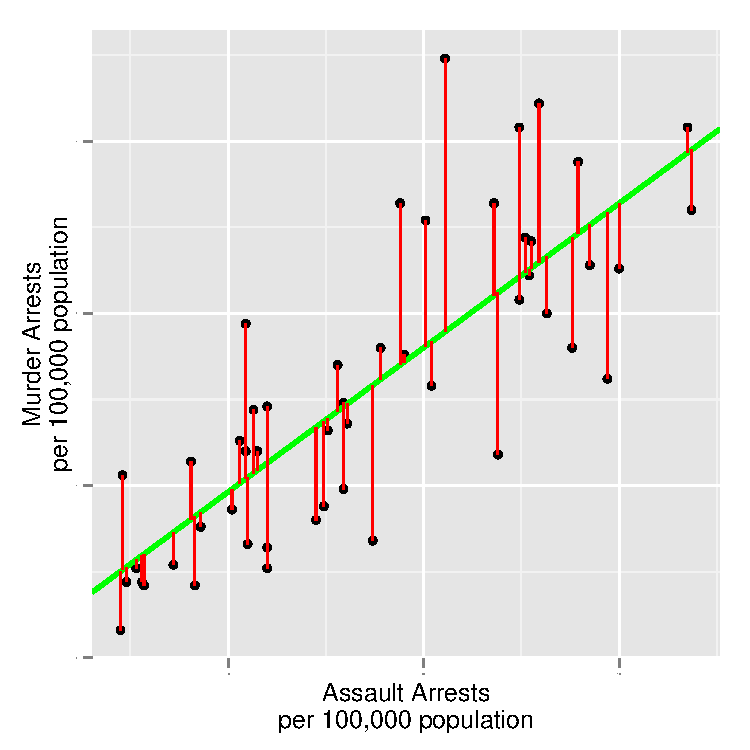
\includegraphics[width=\maxwidth]{figure/graphics-ols-1} 

}

\caption[Green regression line with prediction error, as noted in red on the chart]{Green regression line with prediction error, as noted in red on the chart}\label{fig:ols}
\end{marginfigure}


\end{knitrout}

This is very similar to the traditional algebra formula $y=mx+b$ with slope $m$ and y-intercept $b$. In this case, the slope is $\hat{\beta}$.
\begin{equation*}
\hat{\beta}=\frac{Cov(X,Y)}{Var(X)}=Corr(X,Y)\frac{StdDev(Y)}{StdDev(X)}
\end{equation*}
Note that $\hat{\beta}$ is very close to the correlation value of $\frac{Cov(X,Y)}{StDev(X)StDev(Y)}$, but with $StDev(X)$ replacing $StDev(Y)$, to indicate the dependency of $Y$ upon $X$.

For the US Arrests data set, 
\begin{equation*}
\hat{\beta}=\frac{285.2416}{6806.32}=0.04191
\end{equation*}

The linear regression always goes through the point $(\bar{x},\bar{y})$, so returning to algebra, any point plus the slope determines the line:
\begin{equation*}
\hat{\alpha}=\bar{y}-\hat{\beta}\bar{x}
\end{equation*}

The predicted value for any $y_i$ is $\hat{y_i}$, and the prediction error is $\hat{\epsilon}=y_i - \hat{y_i}$.

Some properties of the Simple Linear Regression:
\begin{itemize}
  \item $\Sigma_{i=1}^{N} \hat{\epsilon}=0 $
  \item $\Sigma_{i=1}^{N} x_i \hat{\epsilon}=0 $
  \item The predicted values $\hat{y_i}$ minimize the sum of the squared prediction errors, $\Sigma_{i=1}^{N} \hat{\epsilon}^2$, often referred to as Sum Squared Errors, or SSE.
  \item The regression equation is valid to predict $\hat{y}$ values in the range of X, that is, on the interval (min(X),max(X)), and any prediction will be in the range of (min(Y),max(Y))
\end{itemize}



\end{document}
